\section{DISTANCE-BASED FUNCTIONAL CLASSIFICATION}\label{distance-based-functional-classification-marie}

There are many downstream analysis tasks in functional data analysis that are based on pairwise distances, including distance-based nonparametric regression and distanced-based functional clustering.
In this section, we explore whether our geodesic distance estimator has
benefits for the downstream analysis task of functional classification. 

We work with the non-parametric classifier proposed in \cite{Ferraty2006} which is a functional version of the Nadaraya-Watson kernel estimator. Given a sample of curves $X_1,\ldots,X_n$ where each function $X_i$ is associated to a class label $Y_i$, the estimator of the probability that a new observation $X^\star$ is in class $Y^\star=y$ is defined as
\begin{equation}\label{func_NW}
\hat P(Y^\star = y | X^\star)= \frac{ \sum_{i=1}^n k[h^{-1} d(X^\star,X_i)] {\bf{1}}(Y_i = y) }{ \sum_{i=1}^n k[h^{-1} d(X^\star,X_i)] },
\end{equation}
where $d$ is a distance, $k$ a kernel, $h$ a bandwidth and $\bf{1}$ the indicator function. The curve $X^\star$ is then classified in the class $Y^\star =y$ for which the conditional probability (\ref{func_NW}) is largest. We compare the classification performance obtained with the distance $d$ given by our proposed geodesic distance with $s=1,2$ and $3$, as well as that given by Spline IsoGeo and Spline L2 described in the simulation study section. We set $k$ to be a quadratic kernel and the bandwidth $h$ is chosen by cross-validation. 

The classification task is performed on the well-known Berkeley growth curves dataset in functional data analysis, available in the \emph{fda} package \cite{Ram-Hoo-Gra} for R \cite{Rproject}. We chose this dataset because we expect the data to contain nonlinear features as suggested in \cite{ChenMuller2012}. The data consist of the height of $n=93$ individuals, 39 boys and 54 girls, measured on a common grid $t_1,\ldots,t_K$ of $K=31$ points taken between the ages of 1 and 18 years. The raw data $Y_1,\ldots,Y_n$ are transformed to continuous functions by smoothing with B-spline bases with a roughness penalty on the fourth derivative :
$$\tilde X_i(t) = \sum_{l=1}^{b} c_{il}B_l(t), $$
where
 \begin{eqnarray*}
 (c_{i1},\ldots,c_{ib})&=&\arg \min_{c\in \R^b}\Bigg\{\sum_{j=1}^K\left(\sum_{l=1}^{b} c_{il}B_l(t_j)-Y_{ij}\right)^2\\
 &&\quad +\lambda \left\|\sum_{l=1}^{b} c_{il}\partial^4_tB_l\right\|^2_{L^2}\Bigg\}.
 \end{eqnarray*} 
We use $b=35$ B-splines bases of order 6 and the parameter $\lambda$ is chosen by generalized cross-validation. We then differentiate the resulting fonctions to obtain velocity curves; the data are illustrated for boys and girls on Figure \ref{fig:data_illu}.





To assess the classification performance of the the proposed geodesic distance, we randomly split $200$ times the dataset into a training set of $50$ curves and a test set of $43$ curves. For each split, we calculate the misclassification error, and we average these errors over the splits. The results are presented in Figure \ref{fig:class_err_velo}, we can see that our method with $s=3$ performs a little bit better than the others and that our method with $s=2$ is equivalent to Spline IsoGeo and Spline L2.

\begin{figure}[t]
\centering
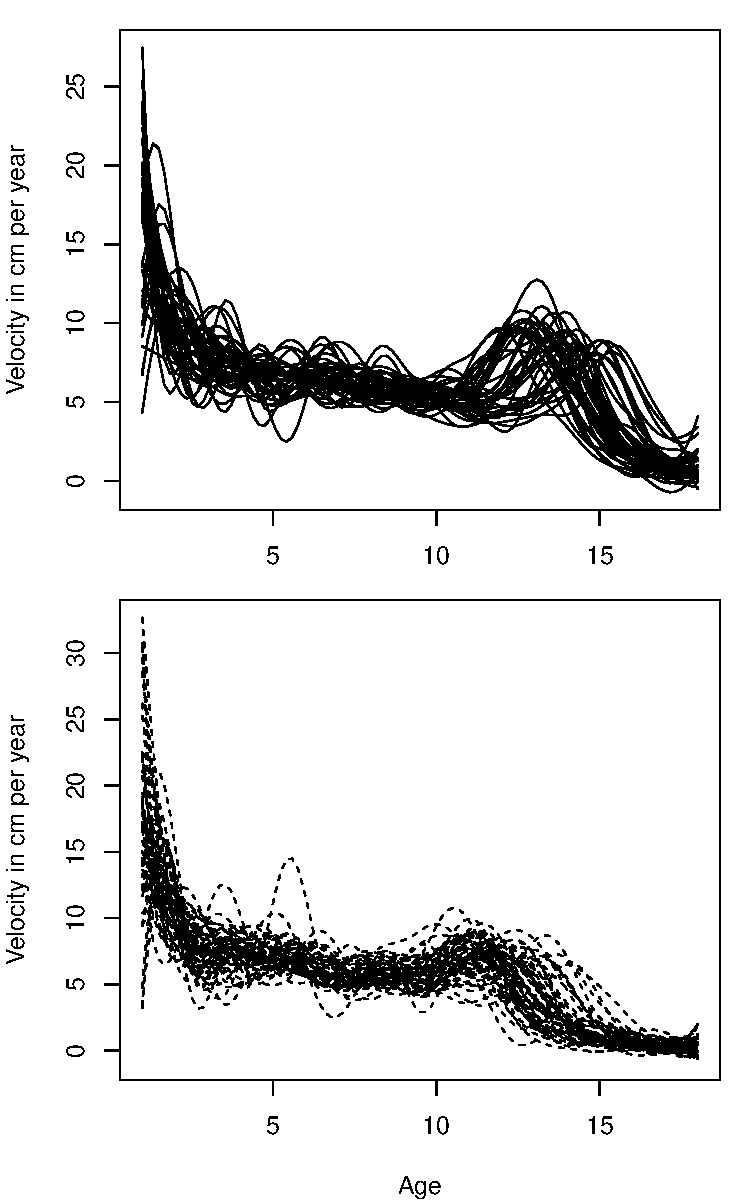
\includegraphics[height=0.5\textheight]{./Velocity_curves_data_illustration.pdf}
\caption{Velocity curves of 39 boys (top) and 54 girls (bottom).}
\label{fig:data_illu}
\end{figure}

\begin{figure}[h!]
\centering
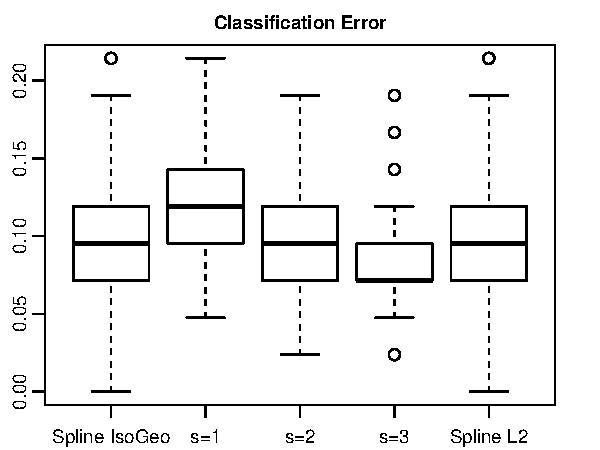
\includegraphics[height=0.3\textheight]{./Erreur_classification_velocity.pdf}
\caption{Classification errors for the velocity curves, our method with $s=3$ performs better while our method with $s=2$ is equivalent to Spline IsoGeo and Spline L2.}
\label{fig:class_err_velo}
\end{figure}


% It must be noted that while
% curve alignment, also known as curve registration, is necessarily
% performed as a preprocessing technique prior to clustering and
% classification, our geodesic distance estimator allows one to forsake
% this step.




 


% For simplicity, assume the task is binary classification. Associated to
% each functional object \(x\) is a binary \(y\) indicating class
% membership. Consider the classifier proposed in \cite{Ferraty2006} which
% is a functional version of the Nadaraya-Watson kernel estimator of class
% membership probabilities: \[
% \hat p(y = 0 | x) \frac{ \sum_{i=1}^n K[h^{-1} d(x,x_i)] 1(y_i = 0) }{ \sum_{i=1}^n K[h^{-1} d(x,x_i)] }
% \] We shall compare our method to using \(L^2\) distance, possibly
% weighted, and with curve registration already accomplished. Describe
% alternative methods in detail.
% 
% The bandwidth in the classifier should be tuned individually for each
% method. Also we might need to tune MDS dimension \(s\) since in real
% data, the dimension of the manifold might be much higher than
% encountered in the simulation scenarios where it never goes above 2.

% Datasets used by functional classification papers
% 
% \begin{itemize}
% \item Wheat, rainfall and phoneme in Aurore's paper "Achieving near-perfect classification for functional data"
% \item Berkeley growth curves in \cite{ChenReiss2014}.
% \item Tecator and phoneme in \cite{Galeano2015} Mahalanobis technometrics paper.
% \item yeast cell cycle gene expression (can't find this publicly) in \cite{LengMuller2005} "Classification using functional data analysis for temporal gene expression data"
% \end{itemize}
% 
% Datasets used in functional manifold papers
% 
% \begin{itemize}
% \item Berkeley growth, yeast cell cycle gene expression (can't find this publicly) in \cite{ChenMuller2012}
% \item Tecator in \cite{LinYao2017} contamination paper
% \item Berkeley growth, gait cycle in \cite{Dimeglio2014} robust isomap paper
% \end{itemize}
